\documentclass[10pt]{article}
\usepackage{amsmath,textcomp,amssymb,geometry,graphicx,enumerate,tikz,algorithm,algpseudocode,pifont,upgreek}
\usetikzlibrary{calc}
\usetikzlibrary{datavisualization}
\usetikzlibrary{datavisualization.formats.functions}


\textheight=9in
\textwidth=7in
\topmargin=-.75in
\oddsidemargin=-0.25in
\evensidemargin=-0.25in

\usepackage{listings}
\lstnewenvironment{codeblock}
    {\lstset{language=Python,
      showspaces=false,
      showtabs=false,
      breaklines=true,
      mathescape=true,
      showstringspaces=false,
      breakatwhitespace=true,
      commentstyle=\textit,
      keywordstyle=\textbf,
      basicstyle=\ttfamily,
      escapechar=`,
    }}
    {}

\newcommand{\bigo}{\mathcal{O}}
\newcommand{\R}{\mathbb{R}}


\begin{document}
\section*{04/27/2016}
\subsection*{Speeding up NN}
\subsubsection*{Voronoi diagrams}
	\begin{itemize}
		\item Let $P$ be a point set. The \underline{voronoi cell} of $w \in P$ is $Vor w = \{p \in \R^{d}: |pw| \leq |pv| \ \forall v \in P\}$.
		\item The \underline{Voronoi diagram} of $P$ is the set of all $P's$ voronoi cells.
		\item Size (e.g. \# of vertices) $\in \bigo(n^{\lceil \frac{d}{2}\rceil})$ .. but often in practice is in $\bigo(n)$.
		\item \underline{Point location}: Given query point $v$, find the point $w$ for which $v \in Vor w$.
		\item 2D: $\bigo(n\log n)$ time to compute V.d. and a \underline{trapezoidal map} for point location. $\bigo(\log n)$ query time.
		\item dD: Use \underline{binary space partition tree} (BSP tree) for point location.
		\item 1-NN only! What about k-NN?
		\item \underline{order-k voronoi diagram} has a cell for each possible combination of k-NN.
		\item In 2D, size $\in \bigo(k^{2}n)$.
	\end{itemize}

\subsubsection*{k-d Trees}
\begin{itemize}
	\item Decision trees for NN search. Differences:
		\begin{itemize}
			\item No entropy. Split dimension w/greatest variance or width (max-min).
			\item Each internal node stores a sample point.
		\end{itemize}
		\begin{center}
			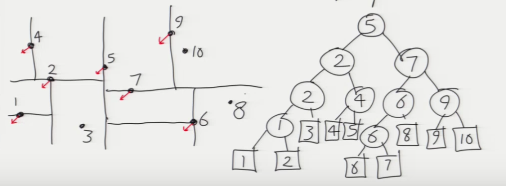
\includegraphics{../images/kdtrees}
		\end{center}
	\item Given query point $q$, find a sample point $p$ such that $|qp| \leq (1 + \epsilon)|qs|$ where $s$ is the closest point.
	\item The algorithm maintains:
		\begin{itemize}
			\item Nearest neighbor found so far (or $k$ nearest)
			\item Heap of unexplored subtrees, keyed by distance from $q$.
		\end{itemize}
		\begin{center}
			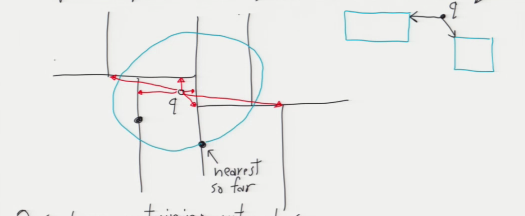
\includegraphics{../images/treekd}
		\end{center}
\begin{codeblock}
    $Q \leftarrow$ heap containing root node of tree
    $r \leftarrow \infty$
    while $Q$ has a cell closer to $q$ than $\frac{r}{1+\epsilon}$:
        $C \leftarrow removeMin(Q)$
        $p \leftarrow C's$ sample point
        $r \leftarrow \min \{r, |qp|\}$
        $C', C'' \leftarrow $ child cells of $C$
        $insert(Q, C')$
        $insert(Q, C'')$
    return point that determined $r$	
\end{codeblock}
	\begin{center}
		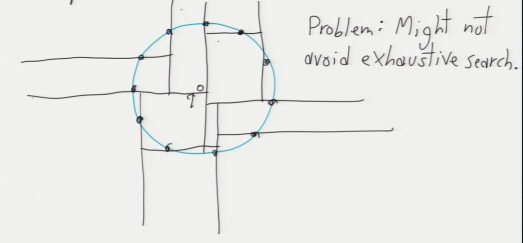
\includegraphics[scale=0.6]{../images/treekd2}
	\end{center}
	\item For k-NN, replacing "r" w/a max-heap holding the k nearest neighbors.
	\item Works w/any $L_{p}-$norm for $p \in [1,\infty]$.
	\item Software:
		\begin{itemize}
			\item ANN (David Mount, and Sunil Aryan, U. Maryland)
			\item FLANN (Marius Muja and David Lowe, U. British Columbia)
			\item GeRaF (Georgios Samaras, U. Athens)
		\end{itemize}
\end{itemize}
\end{document}










